
\documentclass[twoside,12pt, a4paper]{report}

\usepackage[french]{babel}
\usepackage[utf8]{inputenc}
\usepackage{amsmath}
\usepackage{graphicx}
\setlength {\marginparwidth }{2.5cm}
\usepackage[left=3cm,right=3cm,top=2.5cm]{geometry}
\usepackage{float}
\usepackage{titlesec}
\usepackage{forest}
\usepackage{listings}
\usepackage{color}
\usepackage{eurosym}
\usepackage{ftnxtra}
\usepackage[fencedCode]{markdown}
\usepackage[T1]{fontenc}
\usepackage[colorinlistoftodos]{todonotes}
\usepackage{minted}
\usepackage{fnpos}
\usepackage[ruled,vlined]{algorithm2e}
\definecolor{dkgreen}{rgb}{0,0.6,0}
\definecolor{gray}{rgb}{0.5,0.5,0.5}
\definecolor{mauve}{rgb}{0.58,0,0.82}
\usepackage{hyperref}
\hypersetup{linktocpage}



\urlstyle{same}


\setcounter{secnumdepth}{4}

%\usepackage{biblatex} %Imports biblatex package
\usepackage[
    backend=biber,
    style=numeric,
    sortlocale=fr_FR,
    natbib=true,
    url=false,
    doi=true,
    eprint=false
]{biblatex}
\addbibresource{references.bib} %Import the bibliography file



\definecolor{darkWhite}{rgb}{0.94,0.94,0.94}
 
\lstset{
  aboveskip=3mm,
  belowskip=-2mm,
  backgroundcolor=\color{darkWhite},
  basicstyle=\footnotesize,
  breakatwhitespace=false,
  breaklines=true,
  captionpos=b,
  commentstyle=\color{red},
  deletekeywords={...},
  escapeinside={\%*}{*)},
  extendedchars=true,
  framexleftmargin=16pt,
  framextopmargin=3pt,
  framexbottommargin=6pt,
  frame=tb,
  keepspaces=true,
  keywordstyle=\color{blue},
  language=C,
  literate=
  {²}{{\textsuperscriptS}}1
  {⁴}{{\textsuperscript{4}}}1
  {⁶}{{\textsuperscript{6}}}1
  {⁸}{{\textsuperscript{8}}}1
  {€}{{\euro{}}}1
  {é}{{\'e}}1
  {è}{{\`{e}}}1
  {ê}{{\^{e}}}1
  {ë}{{\¨{e}}}1
  {É}{{\'{E}}}1
  {Ê}{{\^{E}}}1
  {û}{{\^{u}}}1
  {ù}{{\`{u}}}1
  {â}{{\^{a}}}1
  {à}{{\`{a}}}1
  {á}{{\'{a}}}1
  {ã}{{\~{a}}}1
  {Á}{{\'{A}}}1
  {Â}{{\^{A}}}1
  {Ã}{{\~{A}}}1
  {ç}{{\c{c}}}1
  {Ç}{{\c{C}}}1
  {õ}{{\~{o}}}1
  {ó}{{\'{o}}}1
  {ô}{{\^{o}}}1
  {Õ}{{\~{O}}}1
  {Ó}{{\'{O}}}1
  {Ô}{{\^{O}}}1
  {î}{{\^{i}}}1
  {Î}{{\^{I}}}1
  {í}{{\'{i}}}1
  {Í}{{\~{Í}}}1,
  morekeywords={*,...},
  numbers=left,
  numbersep=10pt,
  numberstyle=\tiny\color{black},
  rulecolor=\color{black},
  showspaces=false,
  showstringspaces=false,
  showtabs=false,
  stepnumber=1,
  stringstyle=\color{gray},
  tabsize=4,
  title=\lstname,
}

\lstdefinestyle{frameStyle}{
    basicstyle=\footnotesize,
    numbers=left,
    numbersep=20pt,
    numberstyle=\tiny\color{black}
}





\titleformat{\paragraph}
{\normalfont\normalsize\bfseries}{\theparagraph}{1em}{}
\titlespacing*{\paragraph}
{0pt}{3.25ex plus 1ex minus .2ex}{1.5ex plus .2ex}

\begin{document}
\begin{titlepage}
\newcommand{\HRule}{\rule{\linewidth}{0.5mm}} % Defines a new command for the horizontal lines, change thickness here

\center % Center everything on the page
 
%----------------------------------------------------------------------------------------
%	HEADING SECTIONS
%----------------------------------------------------------------------------------------

\textsc{\LARGE Université Libre de Bruxelles}\\[1.5cm] % Name of your university/college
\textsc{\Large }\\[0.5cm] % Major heading such as course name

%----------------------------------------------------------------------------------------
%	TITLE SECTION
%----------------------------------------------------------------------------------------

\HRule \\[0.4cm]
{ \huge D \bfseries }\\[0.4cm] % Title of your document
\HRule \\[1.2cm]
 
%----------------------------------------------------------------------------------------
%	AUTHOR SECTION
%----------------------------------------------------------------------------------------

\begin{minipage}{0.4\textwidth}
\begin{flushleft} \large
\emph{Authors:}\\
Soufiane \textsc{AJOUAOU}\\  000459811\\


\end{flushleft}
\end{minipage}
~
\begin{minipage}{0.5\textwidth}
\begin{flushright} 
\emph{Supervisors:} \\
 \textsc{}\\


\end{flushright}
\end{minipage}\\[2cm]

% If you don't want a supervisor, uncomment the two lines below and remove the section above
%\Large \emph{Author:}\\
%John \textsc{Smith}\\[3cm] % Your name

%----------------------------------------------------------------------------------------
%	DATE SECTION
%----------------------------------------------------------------------------------------

{\large \today}\\[1cm] % Date, change the \today to a set date if you want to be precise

%----------------------------------------------------------------------------------------
%	LOGO SECTION
%----------------------------------------------------------------------------------------


\includegraphics[width=3.3cm, height=3.3cm]{sceau-a-quadri.jpg}%% Include a department/university logo - this will require the graphicx package
 
%----------------------------------------------------------------------------------------

\end{titlepage}

\tableofcontents
\newpage

\chapter{Introduction}
In the domain of cartography, the challenge of simplifying complex geographical data for clear and effective representation has grown increasingly important. As our reliance on automated cartography powered by computer technologies continues to expand, the demand for efficient algorithms becomes ever more critical, particularly in the realms of feature extraction and simplification. Among these algorithms, the Douglas-Peucker line simplification method has remained a foundational tool for representing linear features.

This research is dedicated to extending the frontiers of cartographic representation, with a primary focus on POSTGIS and MobilityDB \cite{zimanyi2019mobilitydb}, by transforming the Douglas-Peucker algorithm into a streaming paradigm. Unlike the traditional application of Douglas-Peucker on static datasets, a streaming algorithm processes data dynamically and continuously, making it ideally suited for real-time or rapidly evolving input. This dynamic adaptability is crucial in modern applications such as GPS navigation, real-time geospatial data analysis, and the constant monitoring of geospatial data streams, all of which are integral to the POSTGIS and MobilityDB ecosystem.

In this study, our paramount objective is the simplification of line representations of mobility data within the POSTGIS and MobilityDB environment. This entails processing an ordered set of n+1 points in a plane, forming a polygonal path comprised of line segments, and deriving a streamlined path with fewer segments while retaining the essential characteristics of the original path. The key distinction here is that our research focuses on the streaming nature of the data, aligning seamlessly with the principles and capabilities of POSTGIS and MobilityDB.

An underlying assumption for this work is the simplicity of the provided path, with an absence of self-intersections. The presence of self-intersections in cartographic data often indicates issues related to digitization errors. While we aspire to maintain the simplicity of the resultant approximation, the question of computational feasibility within the POSTGIS and MobilityDB environment remains a central theme.

The concept of "representing well" encompasses a variety of dimensions, including maintaining proximity between the original and simplified paths, minimizing the area between them, integrating critical points from the original path into the simplified version, and optimizing other measures of curve discrepancy. This study builds upon the established foundations of the Douglas-Peucker algorithm and pioneers the integration of stream data processing into the POSTGIS and MobilityDB framework. This innovation opens new horizons in real-time and dynamic cartographic applications, with a key focus on mobility data.

In summary, this thesis embarks on a pioneering journey to generalize the Douglas-Peucker algorithm for streaming line simplification, with a primary emphasis on the POSTGIS and MobilityDB ecosystem. The motivation behind this endeavor is rooted in the ever-growing demand for adapting cartographic methods to real-time data streams, particularly in the context of dynamic geospatial mobility data.

\iffalse
\subsection{Definitions and Key Concepts}
In this subsection, we will establish a foundational understanding of key terms and concepts central to the research presented in this thesis. These definitions are essential for comprehending the context and significance of the study.

\subsubsection{Moving Objects} 

Moving objects refer to entities or points that continuously change their positions in a given space over time. In the context of this research, moving objects represent dynamic or mobile assets, including vehicles, individuals, or any entities with ever-changing spatial coordinates. Understanding the behavior of moving objects is fundamental for the stream algorithm proposed in this study.

\subsubsection{Stream Data} 

Stream data pertains to the continuous and real-time flow of data that arrives sequentially. In the context of this research, stream data represents the dynamic nature of the information being processed. Stream data includes data points, such as the changing positions of moving objects, which are received and processed as they become available over time.


\subsubsection{Polygonal Path} 

A polygonal path is a sequence of line segments connected end-to-end, forming a coherent trajectory or route. In the context of this research, a polygonal path represents the course taken by moving objects, represented as a series of line segments, which is the primary focus of the stream algorithm for simplification.


\subsubsection{Restricted Version} 

A restricted version in this context signifies a specialized or limited form of an algorithm or problem. It is tailored to accommodate specific constraints or requirements pertinent to the application. For example, a restricted version of a line simplification algorithm may be designed to address particular limitations associated with moving objects and streaming data.



\subsubsection{Function Error} 

Function error indicates the degree of discrepancy between an ideal or reference function and an approximation or simplified representation. In the context of line simplification, it quantifies the degree to which the simplified line retains the essential characteristics of the original polygonal path.

\subsubsection{Fréchet Distance} 

The Fréchet distance is a distance metric that quantifies the similarity between two curves or paths. It measures the likeness between the original polygonal path and a simplified path by considering the minimum separation distance between a moving object on each path as they traverse from start to end.


\subsubsection{The Hausdorff Distance} 

The Hausdorff distance is another distance metric used to measure the similarity or dissimilarity between two sets or paths. It calculates the maximum distance from each point in one set to the nearest point in the other set, providing a measure of the dissimilarity between paths.


\subsubsection{Convex Paths} 

Convex paths represent polygonal paths with the property that any line segment connecting two points lies entirely within the convex hull of the points. Convex paths exhibit certain geometric properties that can be advantageous in the context of simplification algorithms.

\subsubsection{XY-Monotone Paths} 

An XY-monotone path is a polygonal path with the characteristic of being monotonic in both the x and y directions. Such paths move in one direction along the x and y axes without backtracking.

\subsubsection{General Paths} 

General paths encompass polygonal paths without specific constraints on their geometry. They may exhibit complex shapes, including non-monotonic behavior, sharp turns, and diverse geometric characteristics.

\fi

\chapter{State of the Art}
In this section, we will provide a literature review on line simplification algorithms, stream processing algorithms and subjects related to the topic of this thesis.

\section{Error Metrics}
\cite{van2017extensive}
In this section we will explain how to compare a trajectory with its simple counterpart in detail. In this study, a trajectory is represented as a polyline P, which is made up of a series of points  $\{p_{1},..., p_{n}\}$, where the points pi are made up of the longitude, latitude, and sample time-stamp, Xi, Yi, and ti, respectively. Approximation A, which is a subset of P, the polyline of the original trajectory, is the name given to the simplified version of a trajectory. Moreover, the original trajectory's p1 and pn must be included in Approximation A. 
In the thesis we will focus on a spatial metrics in order to compare the trajectory and its simple version.  

\subsection{Hausdorff distance}

 \cite{kerkhof2022algorithmic} 
One simple similarity measure for trajectories is the Hausdorff distance. It is a very
general similarity measure that can be used for any two point sets. If we have two
sets of points P and Q, such as two trajectories if we treat them as polygonal curves
and disregard the timestamps, the directed Hausdorff distance from P to Q is equal.
to the Euclidean distance between the point in P that is furthest from any point in
Q, and the point in Q that is closest to that point. Written formally, we get:

$$\overrightarrow{\mathrm{H}}(P, Q)=\max _{p \in P} \min _{q \in Q} \| p-q \| $$

The undirected Hausdorff distance, also just called the Hausdorff distance, is then
the maximum of the directed distances in both directions.

$$\mathrm{H}(P, Q)=\max \{\overrightarrow{\mathrm{H}}(P, Q), \overrightarrow{\mathrm{H}}(Q, P)\} $$


\subsection{Frechet Distance}

 \cite{kerkhof2022algorithmic}
Another trajectory similarity measure that we use often is the Fréchet distance. It
is based on the principle that similar polygonal curves should not just be close in
space, but there should also exist some parametrization of the curves such that if
we traverse both simultaneously we should remain close at all times. Closeness
here is defined as having small Euclidean distance. The trajectories are treated as
polygonal curves and the timestamps are not taken into account. For polygonal
curves/trajectories P and Q, with P and Q probes respectively, the Fréchet distance
is defined as:

$$\mathrm{F}(P, Q)=\inf _{(\sigma, \theta)} \max _{j:[0,1]}\|P(\sigma(j))-Q(\theta(j))\| $$

where  $ \sigma $   and $ \theta  $  are continuous non-decreasing functions from [0, 1] to the real intervals [1, n] and [1,m], respectively.
This is often explained with the following analogy: Suppose someone is walking
their dog. P is the path the owner takes, and Q is the path of the dog. The owner
and dog can change their speed at will, but they cannot go backwards on the path.
The Fréchet distance is then the shortest possible length the dog’s leash can have
for this walk to be possible.
The weak Fréchet distance is similar, but the constraint is dropped that  $ \sigma $    and $ \theta $  
are non-decreasing. Going back to the man-walking-dog analogy this means the
man and dog can freely move backwards and forwards over their path if this results
in a shorter leash being needed. The weak Fréchet distance between curves thus
gives a lower bound for the (strong) Fréchet distance.
The discrete Fréchet distance is a variant where  $ \sigma $    and $ \theta $   are discrete functions
from {0,..., k} to {1,..., n} and {1,...,m} with the property that 
$0 \leq \sigma (i+1)-\sigma    (i) \leq 1$
and $0 \leq  \theta   (i + 1)-\theta   (i) \leq 1$. This has been explained as someone walking a pet frog,
where instead of walking along edges of the polygonal curve, the owner and frog can
only hop from vertex to vertex. The discrete Fréchet distance between two curves
gives an upper bound on their (continuous) Fréchet distance.
As you might expect, computing the exact Fréchet distance between two curves
is not completely straightforward. Alt and Godau \cite{AltGodau} described an approach for
computing this distance. They de $ \sigma $   ne an algorithm for solving a decision variant of
the problem of computing the distance. This algorithm can answer if the Fréchet
distance between two curves is at most some value $ \delta $ . Then they use a technique
called parametric search to  $ \sigma $   nd the minimum value of $ \delta $ .
Their decision algorithm works by constructing what is called a free space diagram
for a value for $ \delta $ .
It consists of a grid of $   (n - 1)  \times  (m - 1)$ cells, where each cell corresponds to a pair
of line segments, one from P and one fromQ. Each column of cells corresponds to an
edge of P and each row corresponds to an edge of Q. For example, the point (2.6, 3.5)
in a free space diagram corresponds to the probe gotten by linearly interpolating
between P’s second and third probes with a $ \lambda $  of 0.6, and the probe gotten by linearly
interpolating between Q’s third and fourth probes with a $ \lambda $  of 0.5. Each cell is divided
into free space and forbidden space. If the Euclidean distance between the curves at a
point is less than or equal to $ \delta $ , the point is in the free space. If the distance is greater
than $ \delta $ , the point lies in the forbidden space. See Figure \ref{fig:fsd}.

\begin{figure}
    \centering
    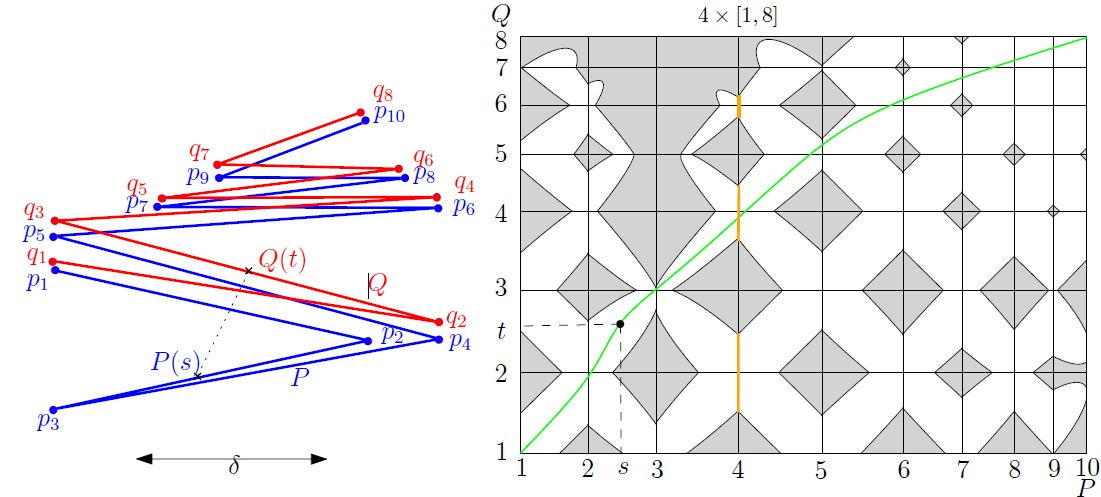
\includegraphics[width=1.0\linewidth]{figures/Figure.jpg}
    \caption{\cite{kerkhof2022algorithmic} Enter Two polygonal curves P (in blue) and Q (in red), and their free space
diagram for the chosen value of  $ \delta $. The free space is shown in white and the forbidden
space is shown in gray. Each cell of the FSD corresponds to the combination of
one edge of P and one edge of Q. (s, t) is a free point in the diagram, lying on a
reachable path in the free space. One green spot is marked in both the FSD and on
the associated spots on P and Q. A x- and y- monotone path contained in the free
space from (1, 1) to (8, 10), shown in green, corresponds to parametrizations of P and
Q realizing a Fréchet distance of at most  $ \delta $.}
    \label{fig:fsd}
\end{figure}

Now, an x- and y-monotone path from the point (1, 1) to (n,m) entirely through
the free space corresponds to parametrizations of P and Q such that the distance
between the two is at most $ \delta $  at any time, i.e. the Fréchet distance is at most $ \delta $ .
For additional details we refer to the paper by Alt and Godau \cite{AltGodau}

\section{Line simplification algorithm}
Line simplification deals with the simplification of arbitrary lines, which can be straight or curved. The goal is to reduce the complexity of lines while still ensuring that the simplified representation captures the main features of the original lines. This algorithm address the problem of Line simplification this problem who is relevant for GPU computing and Spatial Data processing

\subsection{Douglas-Peucker algorithm}
\cite{van2017extensive}
The Douglas-Peucker algorithm  \cite{douglas1973algorithms} \cite{hershberger1994n} takes a polyline
P a sequence of points $\{p_{1},..., p_{n}\}$ , and a user defined
allowed spatial error, $\varepsilon$ > 0. The algorithm builds an
approximation polyline $P'$ , initially consisting of $p_{1}$ and
$p_{n}$. It continues adding the point pi out of the original
polyline that has the largest shortest-euclideandistance
to $P'$ until that distance is smaller than $\varepsilon$ as
demonstrated in Figure \ref{fig:dgpk}.

\begin{figure}
    \centering
    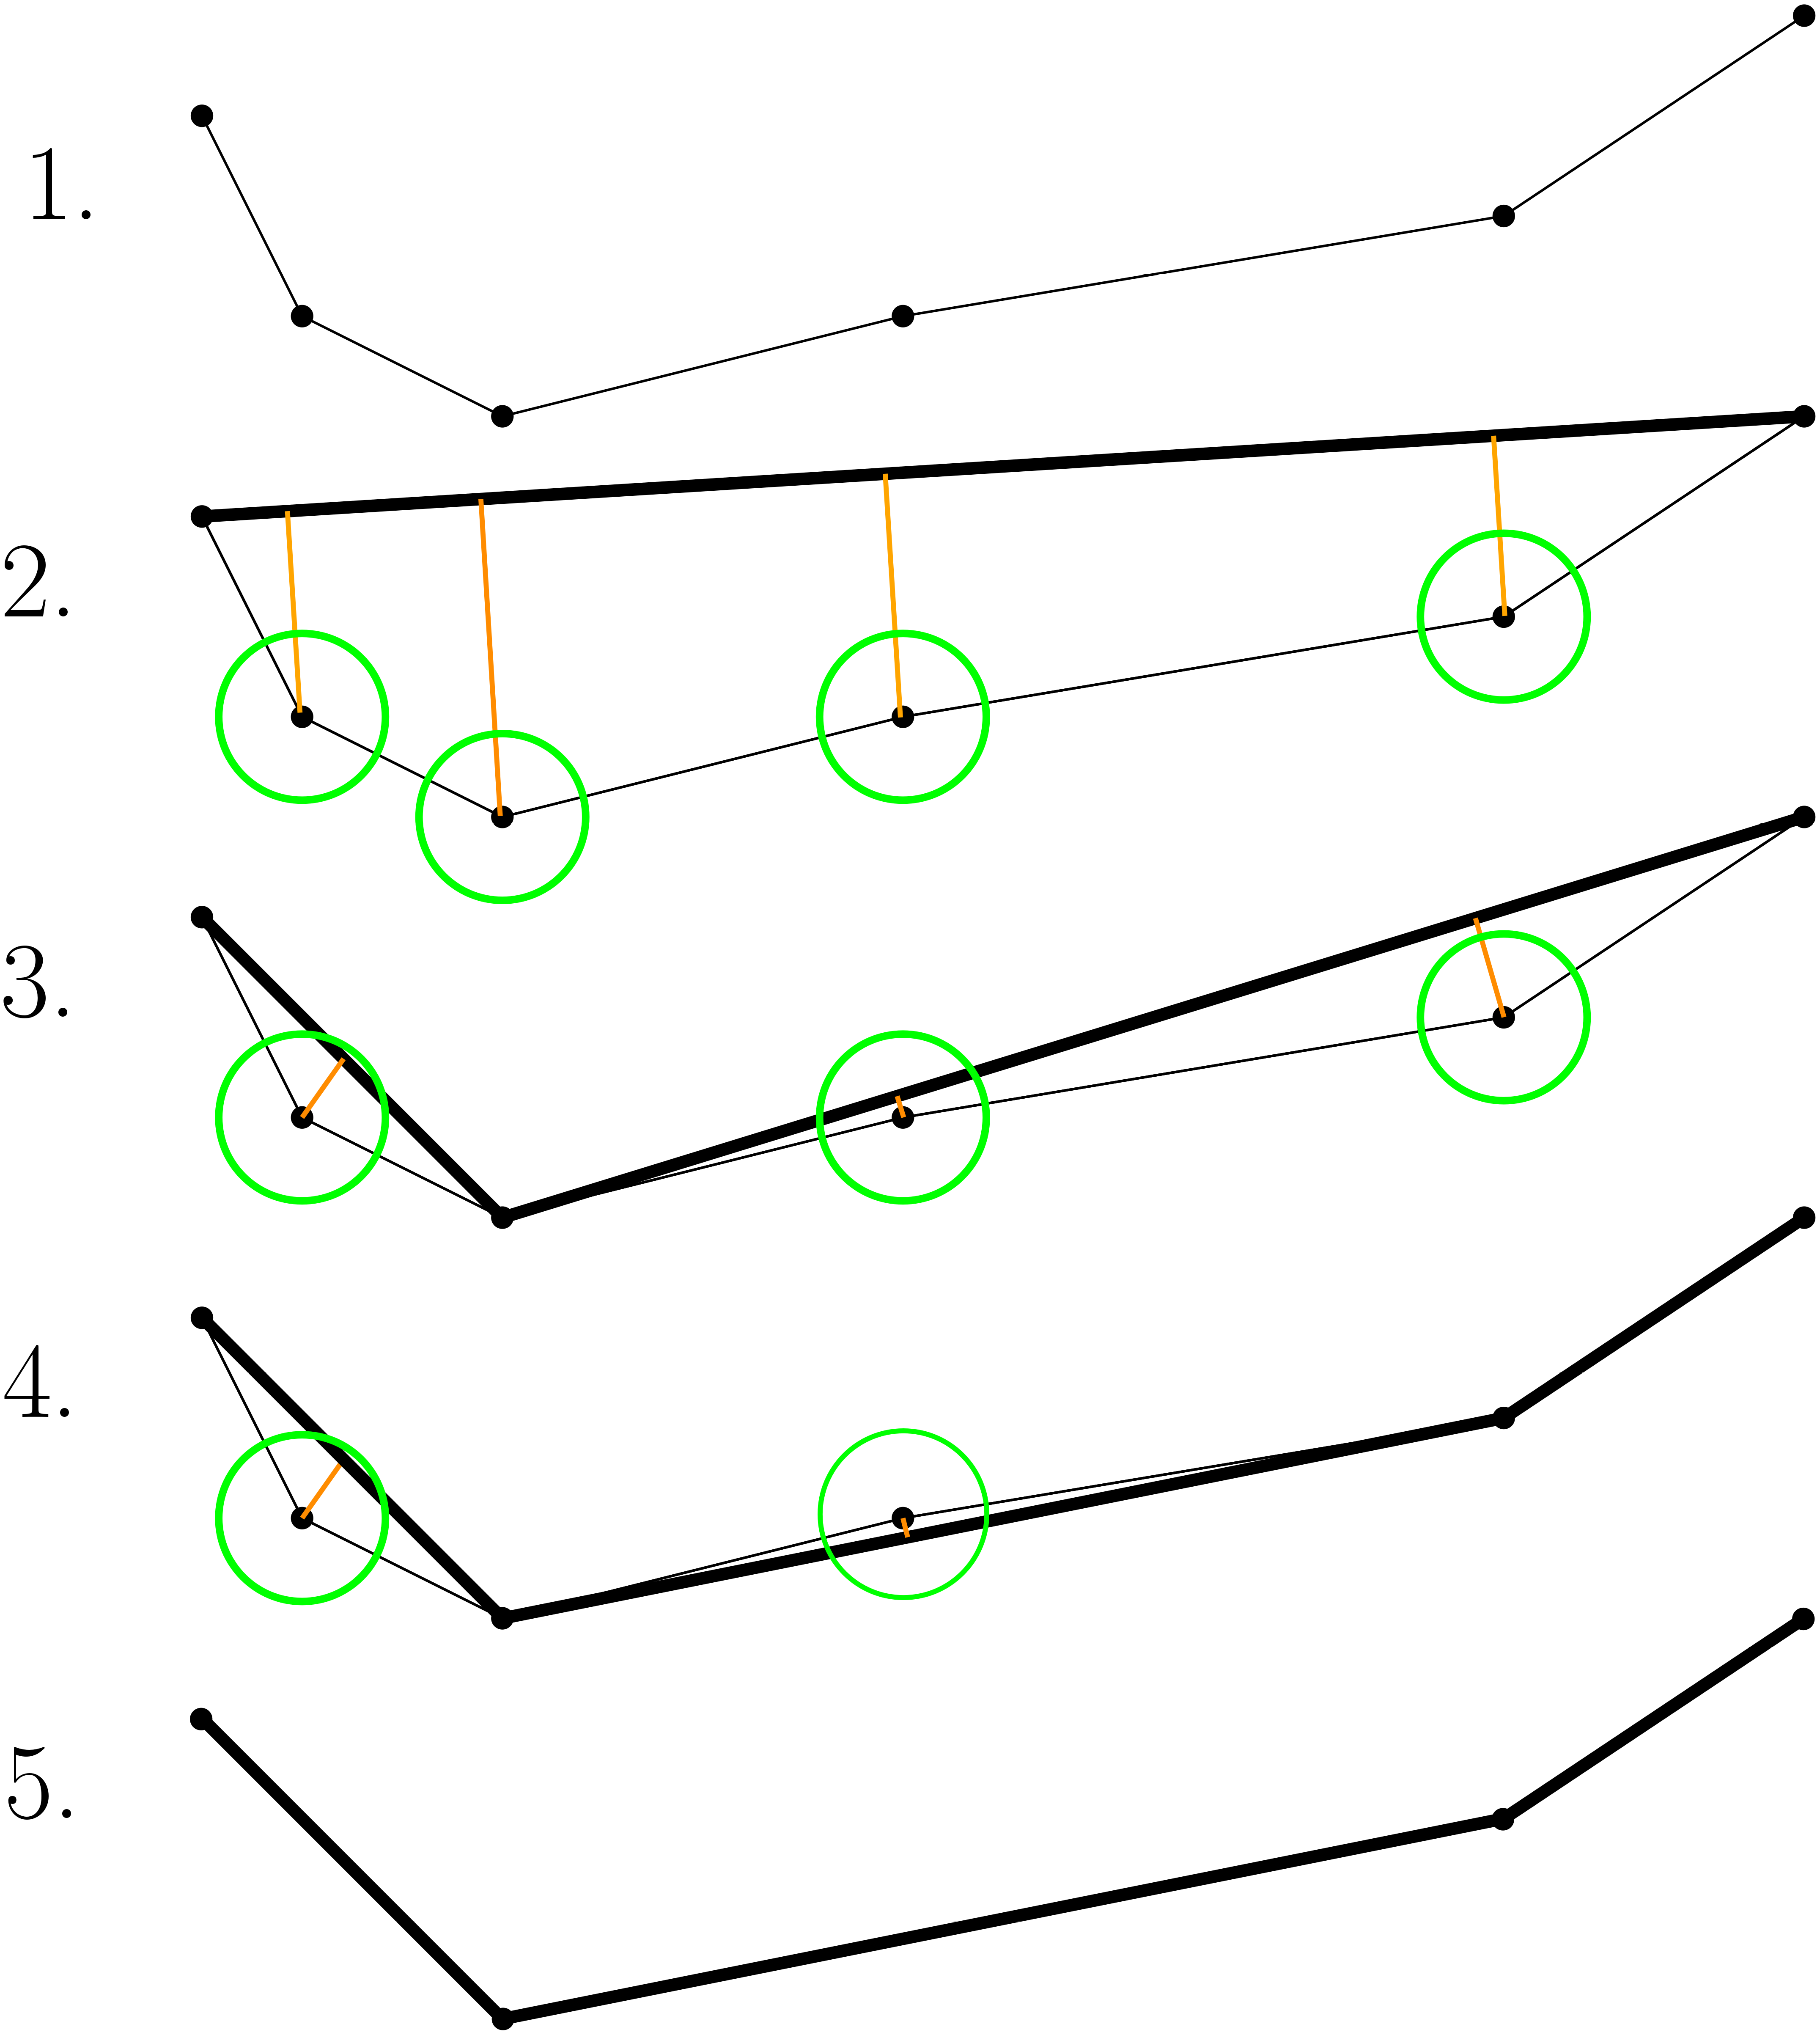
\includegraphics[width=0.5\linewidth]{figures/dgpk.png}
    \caption{\cite{van2017extensive} Illustration of how the Douglas-Peucker algorithm
iteratively simplifies a line. The allowed spatial
error  $\varepsilon$  is depicted with green circles. }
    \label{fig:dgpk}
\end{figure}

\subsection{Visvalingam-Whyatt algorithm}
\cite{van2017extensive}
The Visvalingam-Whyatt algorithm \cite{doi:10.1179/000870493786962263} uses the concept
of ‘effective area’, which is the area of the triangle
formed by a point and its two neighbors. The algorithm
takes a polyline P a sequence of points $\{p_{1},..., p_{n}\}$, and
a user defined allowed spatial displacement error, $\varepsilon$ > 0.
For every set of three consecutive points $\{p_{i-1},p_{i},p_{i+1}\}$
a triangle is formed with its surface being the ‘effective area’. Iteratively point $p_{i}$ is dropped that results in
the least areal displacement to form an approximation
as illustrated in Figure \ref{fig:visv}. This process halts when the
‘effective area’ is larger than $\varepsilon$.

\begin{figure}
    \centering
    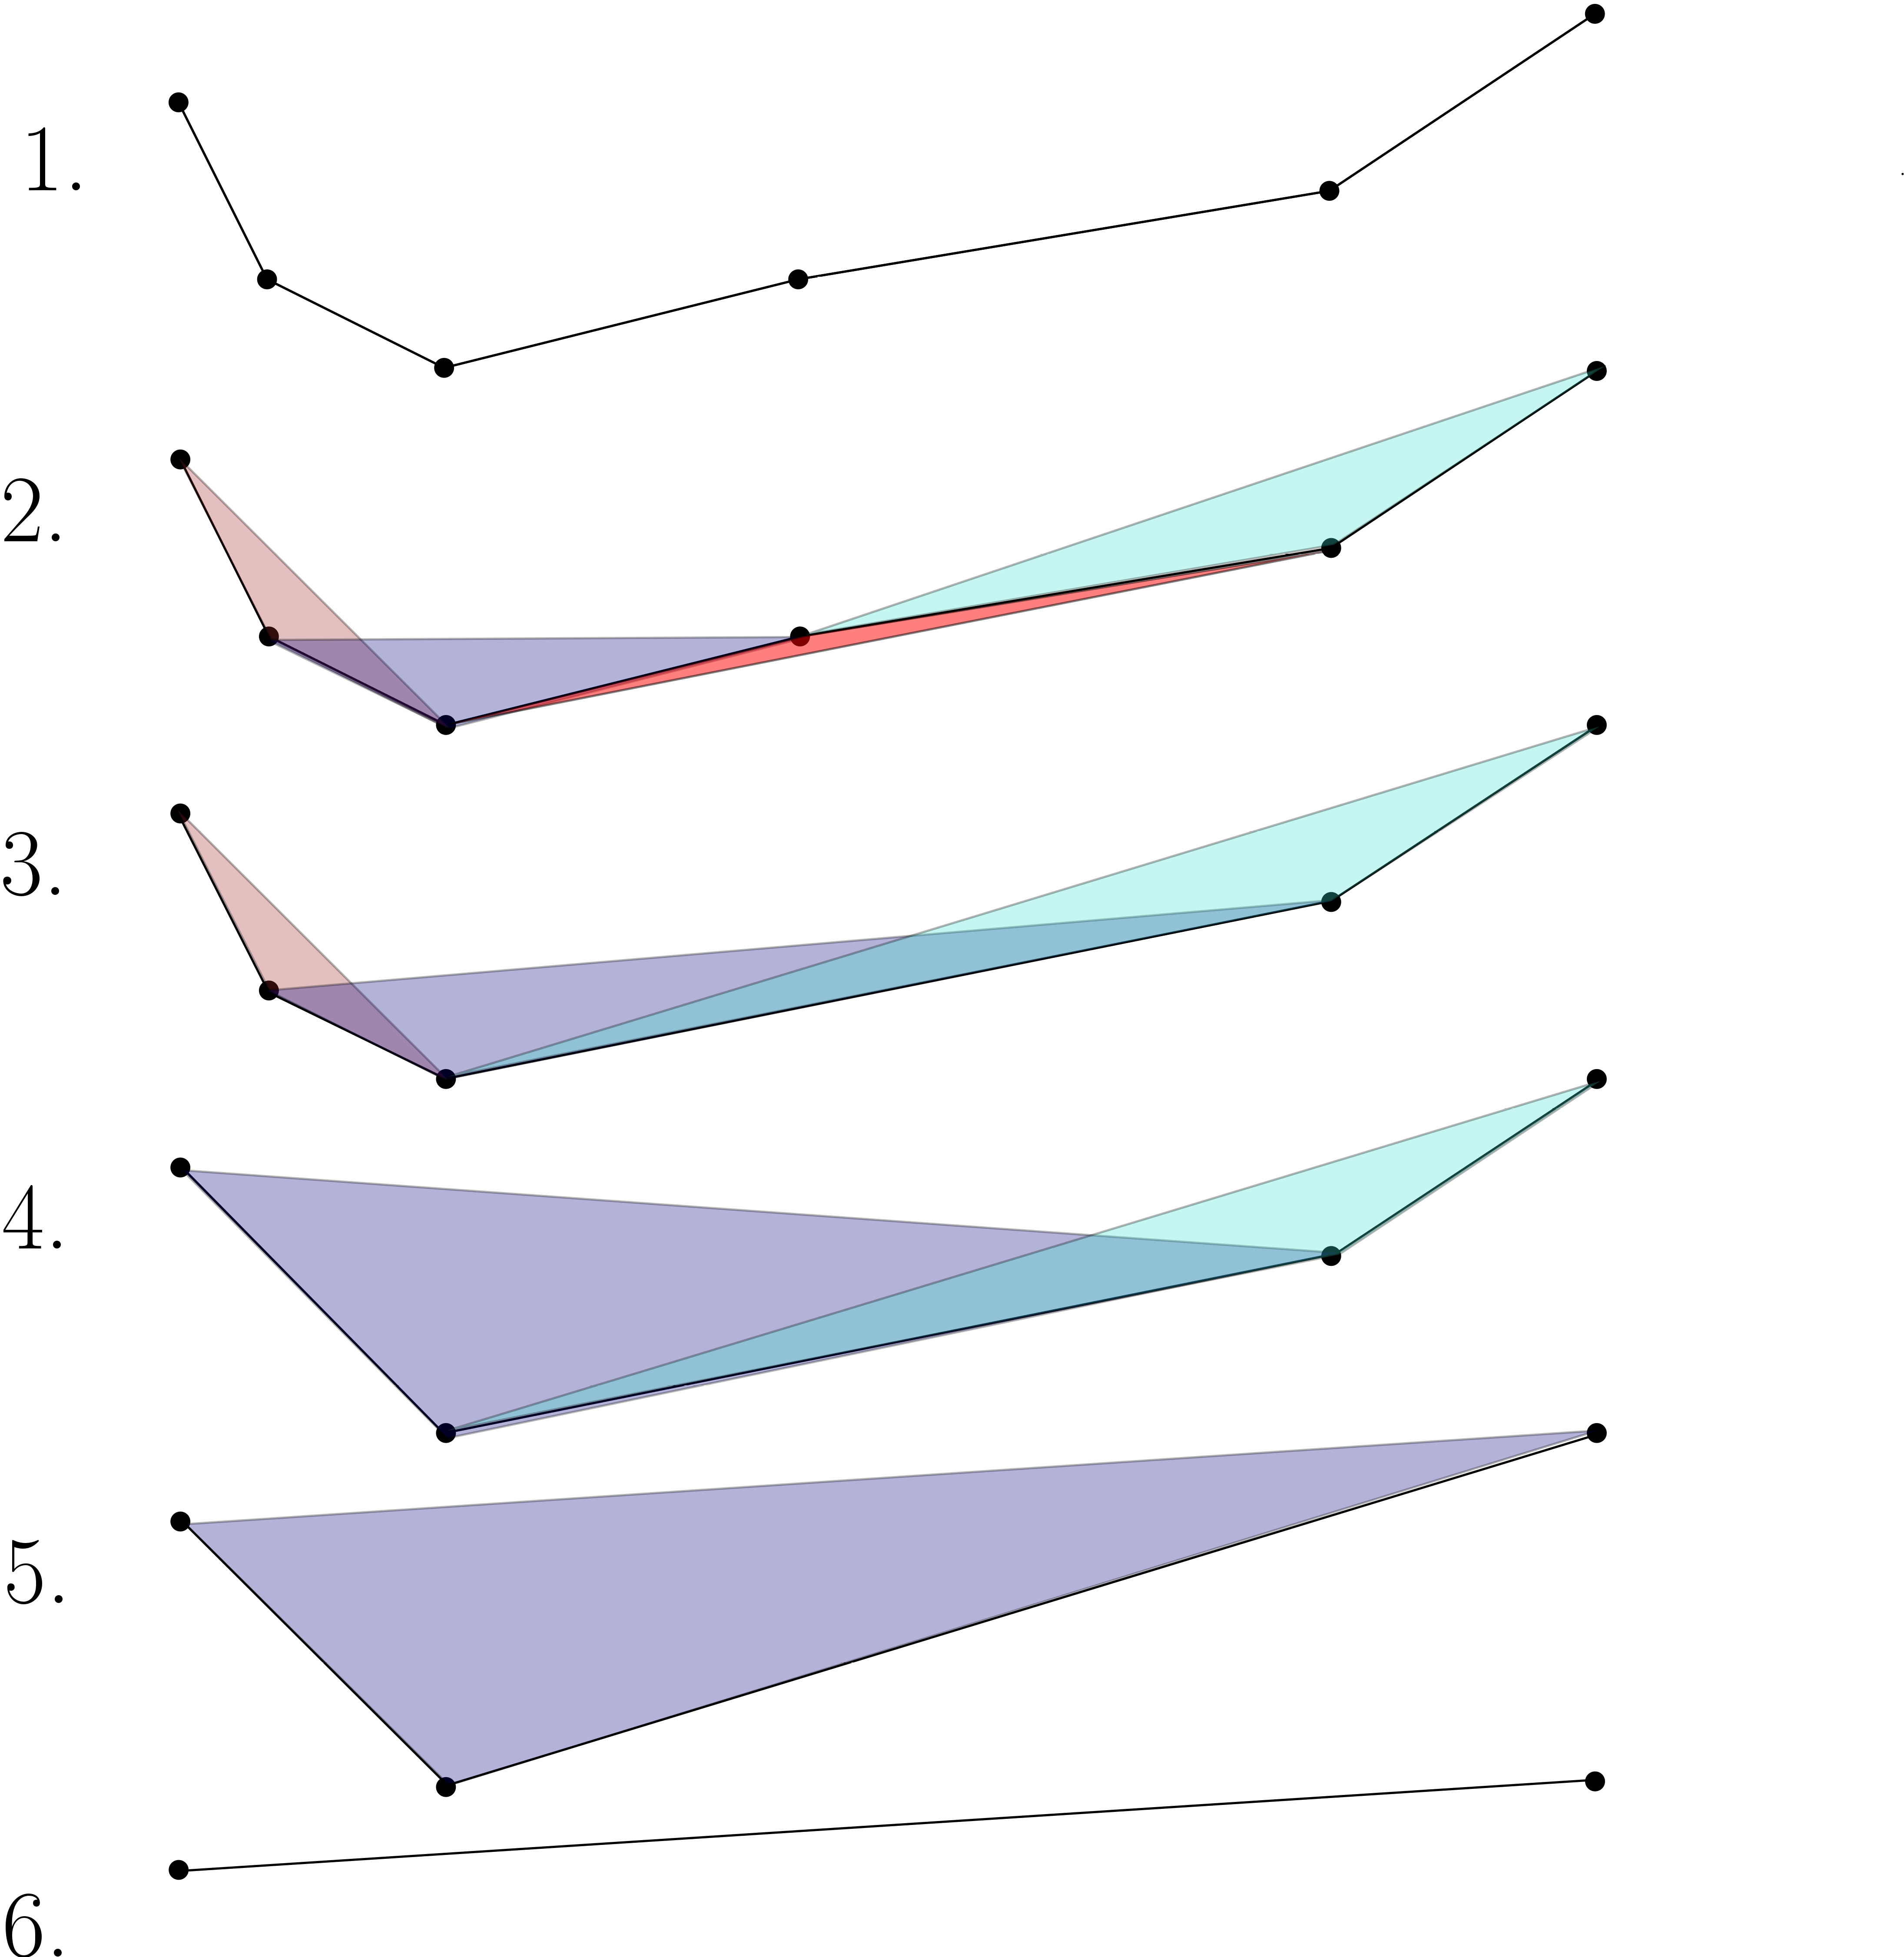
\includegraphics[width=0.5\linewidth]{figures/visv.png}
    \caption{\cite{van2017extensive} Illustration of how the Visvalingam-Whyatt
algorithm iteratively simplifies the line.}
    \label{fig:visv}
\end{figure}

\subsection{Imai-Iri}
\cite{van2017extensive}
The basis of the Imai-Iri algorithm \cite{IMAI198631} lies in the construction
of an unweighted directed acyclic graph G.
This graph is constructed by connecting all combinations
of two points that would create an allowed shortcut.
A breadth-first search is done on this graph to
compute the shortest path connecting the first and last
point, resulting in the approximation.
This algorithm takes a polyline P a sequence of
points $\{p_{1},..., p_{n}\}$, and a user defined allowed spatial
error, $\varepsilon $ > 0. For each combination of two points ($p_{i}$ and $p_{j}$) it checks if a line between them intersects all
circles with radius $\varepsilon $ that center on the points that lie{\tiny {\tiny }}
between them $\{p_{x} > p_{i},p_{x} < p_{j}\}$. When this is the
case, the line $p_{i}p_{j}$ is an allowed shortcut and is added
to the graph G, see Figure \ref{fig:imai}. After all allowed shortcuts
are added to graph G, breadth-first search is done
to find the shortest path through the graph from $p_{1}$ to $p_{n}$.

\begin{figure}
    \centering
    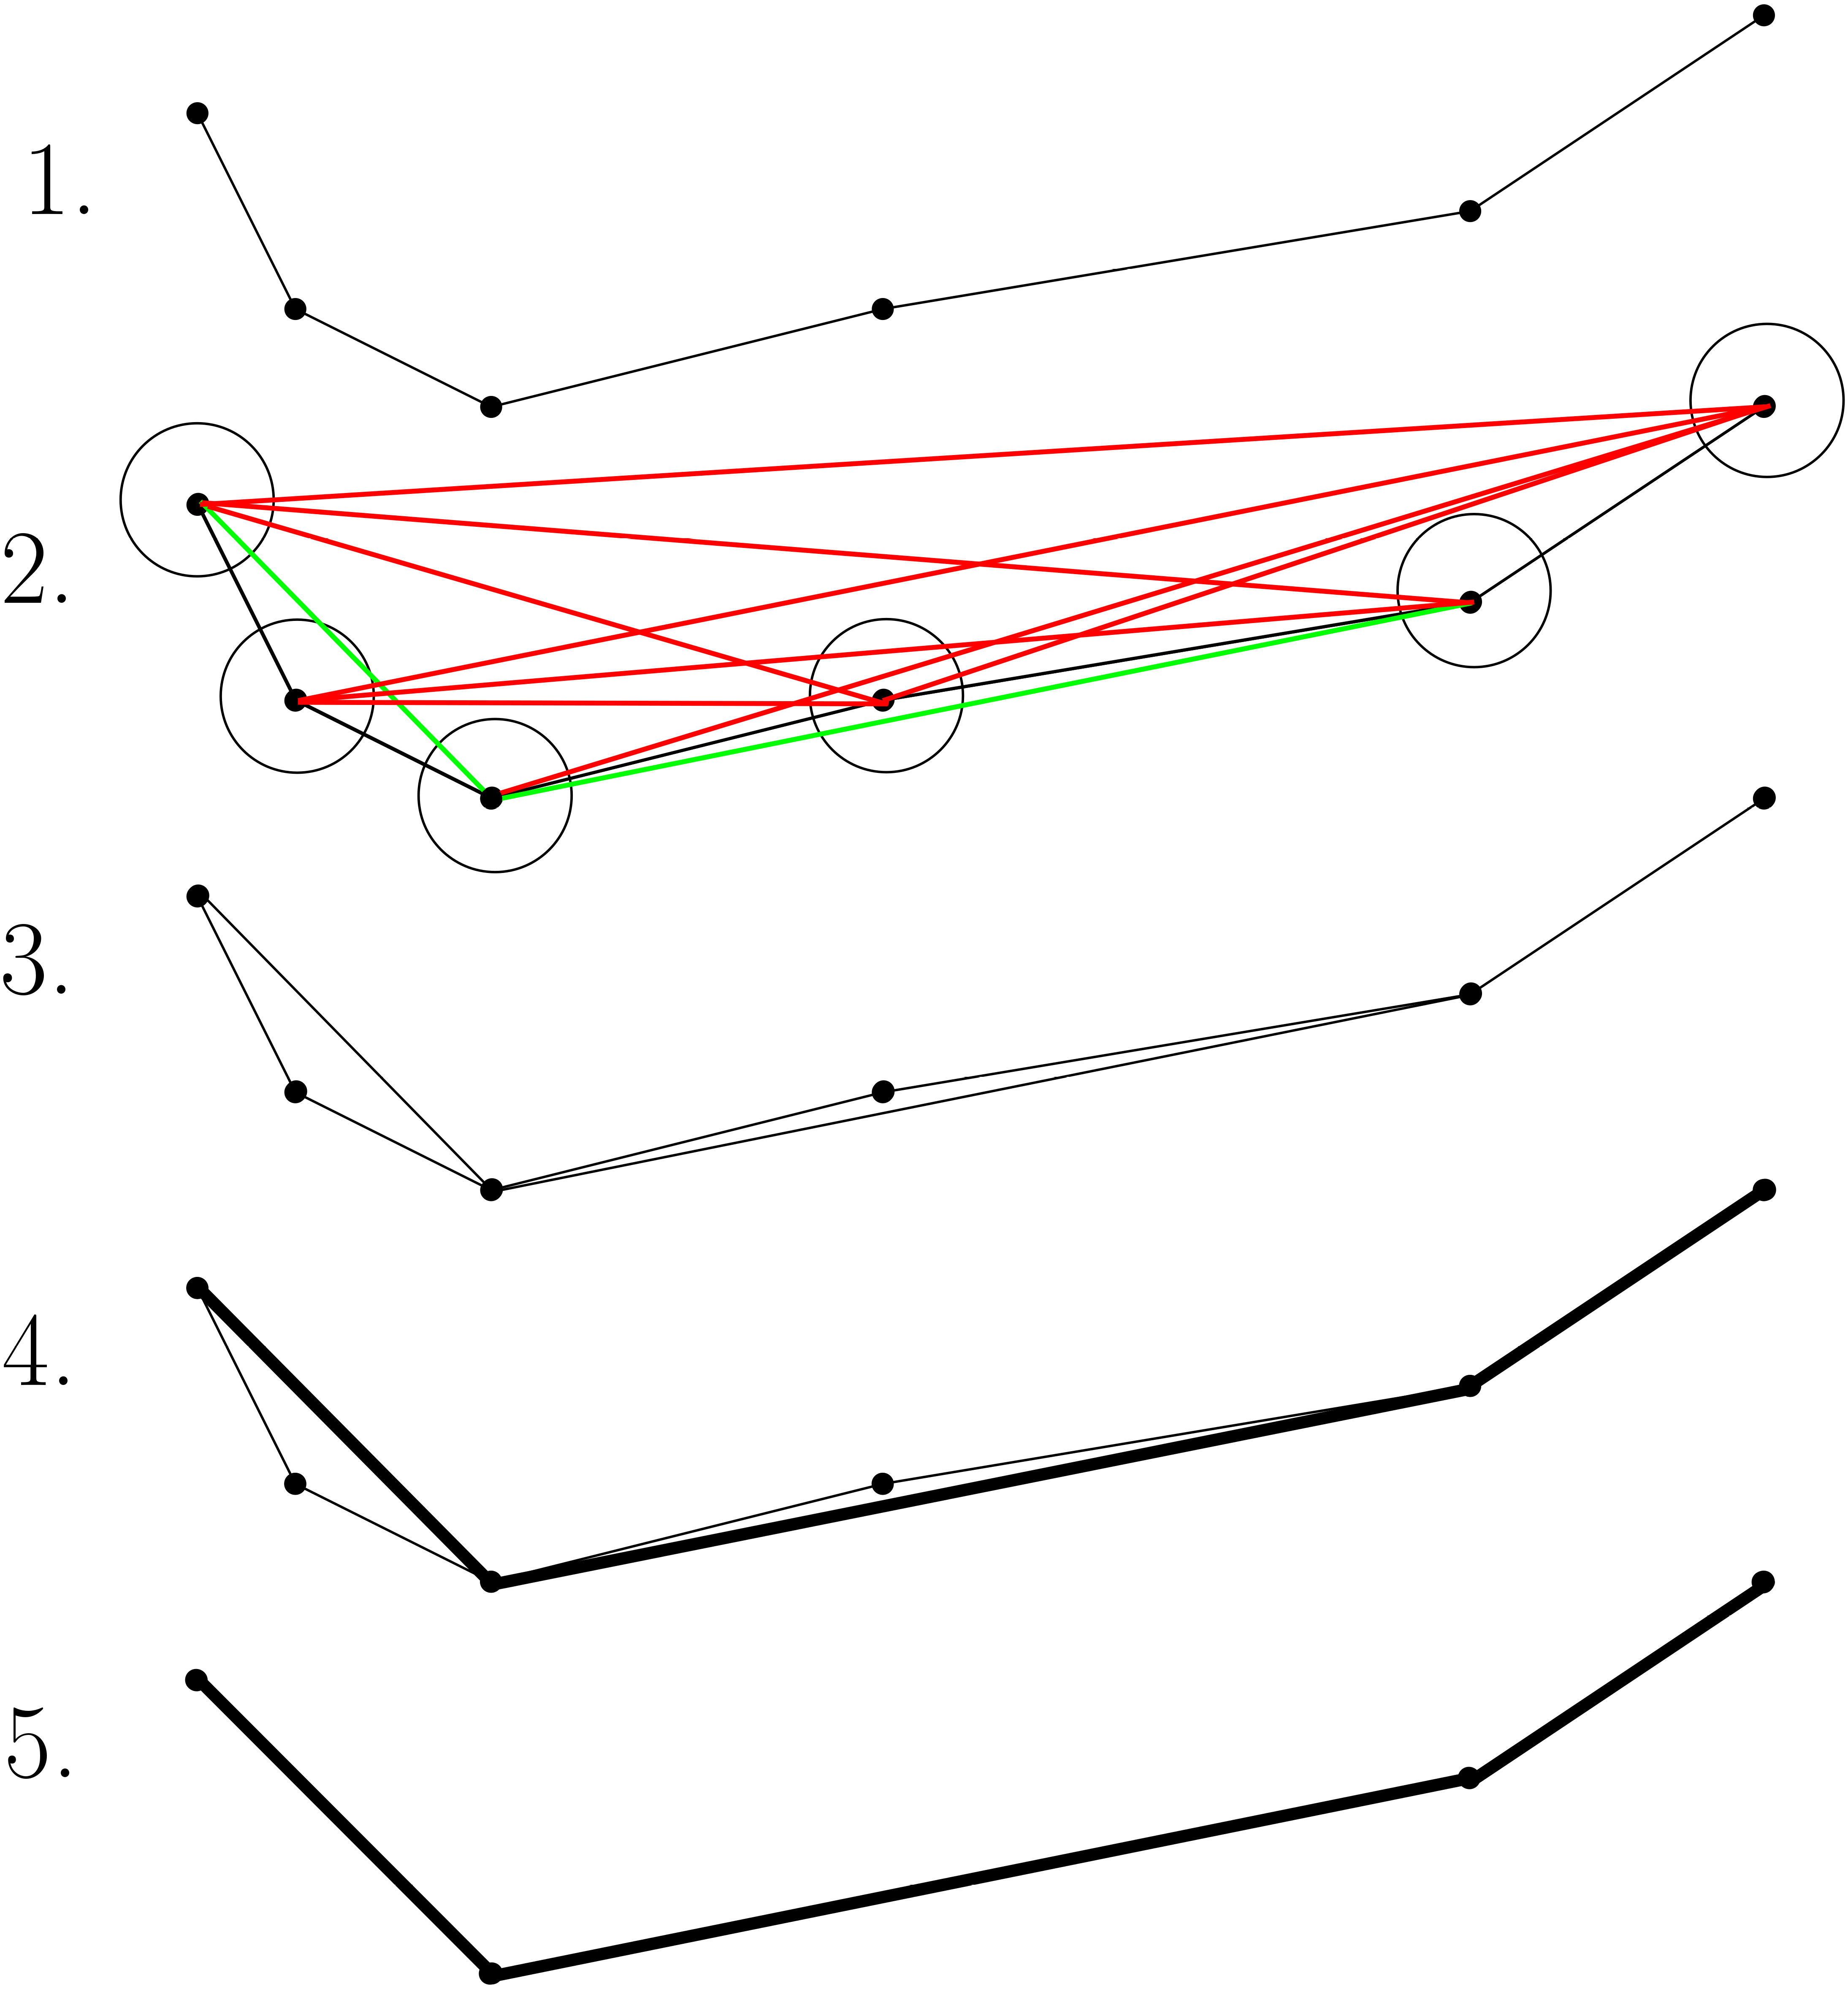
\includegraphics[width=0.5\linewidth]{figures/imaiiri.png}
    \caption{\cite{van2017extensive} Illustration of how the Imai-Iri algorithm generates
shortcuts. Green lines are allowed shortcuts, red
lines are not allowed.}
    \label{fig:imai}
\end{figure}

\section{Streaming Process Algorithm}
\cite{garofalakis2016data}
Traditional data-management systems software is built on the concept of persistent
data sets that are stored reliably in stable storage and queried/updated several
times throughout their lifetime. For several emerging application domains, however,
data arrives and needs to be processed on a continuous (24×7) basis, without
the benefit of several passes over a static, persistent data image. 

It is therefore important to have algorithm to process those stream data.

\subsection{Data-Stream}
\cite{garofalakis2016data}
Perhaps the most basic synopsis of a data stream is a sample of elements from the
stream. A key benefit of such a sample is its flexibility: the sample can serve as input
to a wide variety of analytical procedures and can be reduced further to provide
many additional data synopses. If, in particular, the sample is collected using random
sampling techniques, then the sample can form a basis for statistical inference
about the contents of the stream. Data-stream sampling problems require the application of many ideas and techniques
from traditional database sampling, but also need significant new innovations,
especially to handle queries over infinite-length streams. Indeed, the unbounded
nature of streaming data represents a major departure from the traditional
setting. We draw an important distinction
between a stationary window, whose endpoints are specified times or specified
positions in the stream sequence, and a sliding window whose endpoints move forward
as time progresses. Examples of the latter type of window include “the most
recent n elements in the stream” and “elements that have arrived within the past
hour.” Sampling from a finite stream is a special case of sampling from a stationary
window in which the window boundaries correspond to the first and last stream
elements. When dealing with a stationary window, many traditional tools and techniques
for database sampling can be directly brought to bear. In general, sampling
from a sliding window is a much harder problem than sampling from a stationary
window: in the former case, elements must be removed from the sample as they
expire, and maintaining a sample of adequate size can be difficult.We also consider
“generalized” windows in which the stream consists of a sequence of transactions
that insert and delete items into the window; a sliding window corresponds to the
special case in which items are deleted in the same order that they are inserted.

In the context of this thesis we will investigate the technology of POSTGIS on data stream and adapt the algorithm based on the techniques used by POSTGIS for data stream. 

\subsection{Stream Processing}
\cite{namiot2015big}
Data streams can be generated in various scenarios,
including a network of sensor nodes, a stock market or a
network monitoring system and so on. It exist multiple techniques that could be done on 
a data stream such as continuous queries,clustering,classification,frequent items mining,outlier and anomaly detection.A stream processing solution has to solve different
challenges \cite{Wähner_2014} :
\begin{itemize}
\item  Processing massive amounts of streaming events (filter, aggregate, rule, automate, predict, act, monitor, alert)
\item  Real-time responsiveness to changing market conditions
\item  Performance and scalability as data volumes increase in size and complexity
\item  Rapid integration with existing infrastructure and data sources: Input (e.g. market data, user inputs, files, history data from a DWH) and output (e.g. trades, email alerts, dashboards, automated reactions)
\item  Fast time-to-market for application development and deployment due to quickly changing landscape and requirements
\item  Developer productivity throughout all stages of the application development lifecycle by offering good tool support and agile development
\item  Analytics: Live data discovery and monitoring, continuous query processing, automated alerts and reactions
\item  Community (component / connector exchange, education / discussion, training / certification)
\item  End-user|ad-hoc continuous query access
\item  Alerting
\item  Push-based visualization
\end{itemize}

\subsection{Technologies}
\cite{namiot2015big}
In this section, we discuss some technological solutions for
data streams processing.
Apache Storm is a distributed real-time computation system
for processing large volumes of high-velocity data \cite{jain2014learning}. Is a
distributed real-time computation system for processing fast,
large streams of data. Storm is an architecture based on
master-workers paradigm. So a Storm cluster mainly
consists of a master and worker nodes, with coordination
done by Zookeeper.

Spark Streaming \cite{spark} is an extension of the core Spark API
\cite{shoro2015big} that enables scalable, high-throughput, fault-tolerant
stream processing of live data streams. Data can be ingested
from many sources like Kafka, Flume, Twitter, ZeroMQ,
Kinesis, or TCP sockets, and can be processed using
complex algorithms expressed with high-level functions like
map, reduce, join and window, see Figure \ref{fig:streams}.

\begin{figure}[!h]
    \centering
    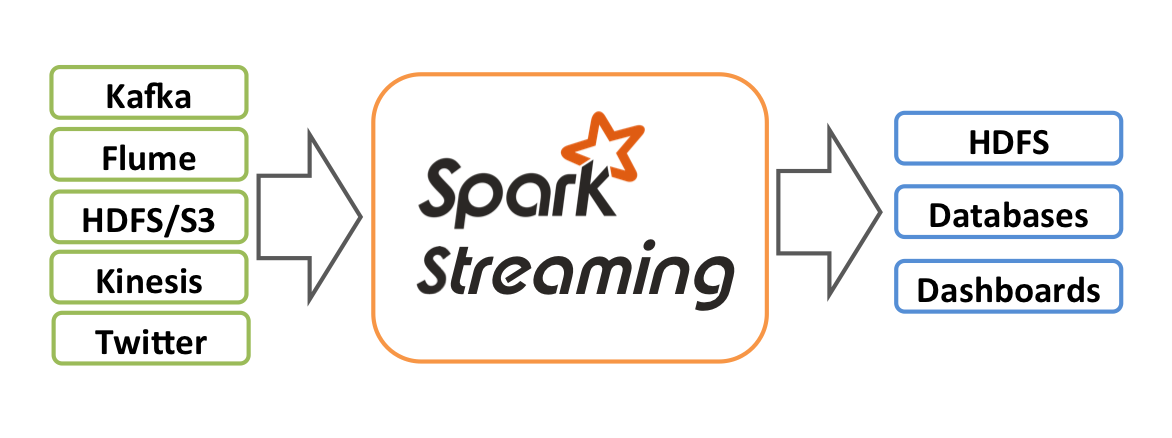
\includegraphics[width=1\linewidth]{figures/streaming-arch.png}
    \caption{\cite{spark} Spark Streaming model representation as we can see it can receive multiple data sources and output to multiple data sources}
    \label{fig:streams}
\end{figure}



Finally, processed data can be pushed out to files systems,
databases, and live dashboards. In fact, you can apply
Spark’s machine learning and graph processing algorithms
on data streams, see Figure \ref{fig:procs}).

\begin{figure}[!h]
    \centering
    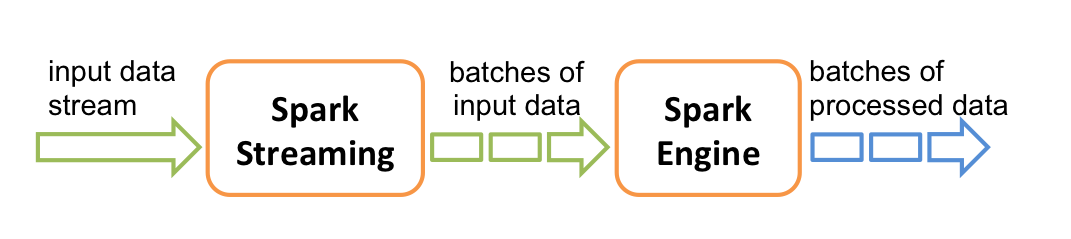
\includegraphics[width=1\linewidth]{figures/streaming-flow.png}
    \caption{\cite{spark} Spark Processing}
    \label{fig:procs}
\end{figure}



\cite{namiot2015big}
Apache Samza \cite{samza} is a distributed stream processing
framework. It uses Apache Kafka for messaging, and
Apache Hadoop YARN to provide fault tolerance, processor
isolation, security, and resource management see Figure \ref{fig:samza}.

\begin{figure}[!h]
	\centering
	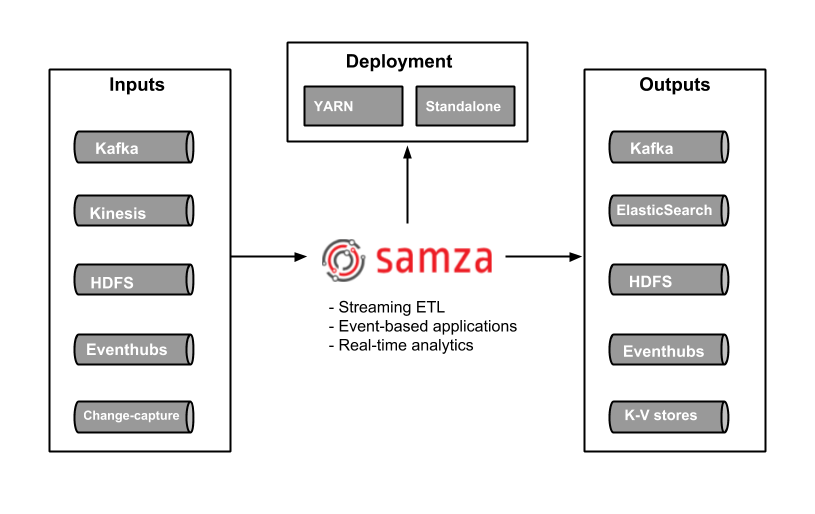
\includegraphics[width=1\linewidth]{figures/samza-arch4.png}
	\caption{\cite{samza} Apache Samza}
	\label{fig:samza}
\end{figure}



Apache Flume \cite{flume} is a distributed, reliable, and available
service for efficiently collecting, aggregating, and moving
large amounts of log data. It has a simple and flexible
architecture based on streaming data flows. It is robust and
fault tolerant with tunable reliability mechanisms and many
failovers and recovery mechanisms. It uses a simple
extensible data model that supports online analytic
applications see Figure \ref{fig:flume}.

\begin{figure}[!h]
	\centering
	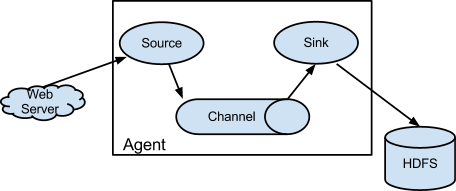
\includegraphics[width=1\linewidth]{figures/DevGuide_image00.png}
	\caption{\cite{flume} Apache Flume}
	\label{fig:flume}
\end{figure}


Apache Kafka itself is often used as a kernel for data stream
architecture. Originally, Apache Kafka is publish-subscribe
messaging rethought as a distributed commit log \cite{ApacheKA}.
Apache Kafka is a distributed system designed for streams.
It is built to be fault-tolerant, high-throughput, horizontally
scalable, and allows geographically distributing data streams
and processing. See Figure \ref{fig:kafka} illustrates stream-centric
architecture in Confluent blog  \cite{Kafka}

\begin{figure}[!h]
	\centering
	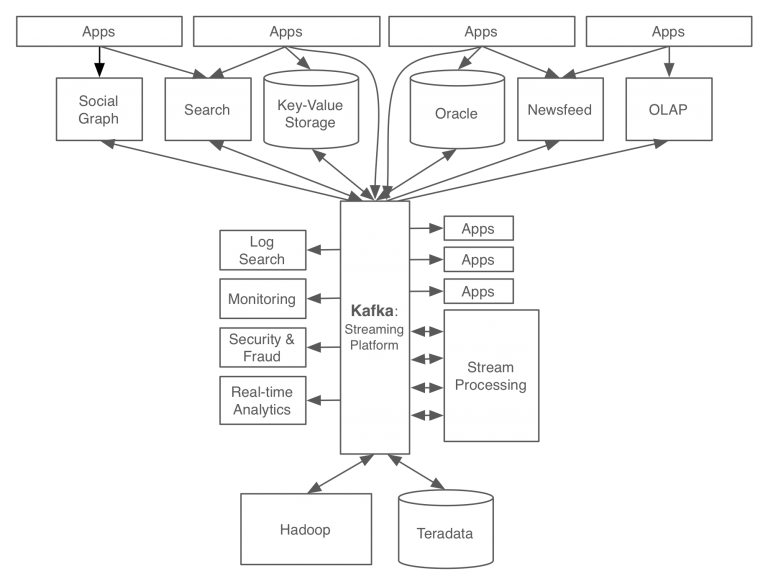
\includegraphics[width=1\linewidth]{figures/data-flow-768x584.png}
	\caption{Stream-centric architecture on Apache Kafka \cite{Kafka} }
	\label{fig:kafka}
\end{figure}

Amazon Kinesis \cite{kinesis} is a fully managed, cloud-based
service for real-time data processing over large, distributed
data streams. Amazon Kinesis can continuously capture and
store terabytes of data per hour from hundreds of thousands
of sources such as website clickstreams, financial
transactions, social media feeds, IT logs, and locationtracking
events.



IBM InfoSphere Streams \cite{ballard2014ibm,ibmdoc} is an advanced analytic
platform that enables the development and execution
of applications that process information in data streams.
InfoSphere Streams enables continuous and fast analysis of massive volumes
of moving data to help improve the speed of business insight and decision making see Figure \ref{fig:ibm}.

\begin{figure}[!h]
	\centering
	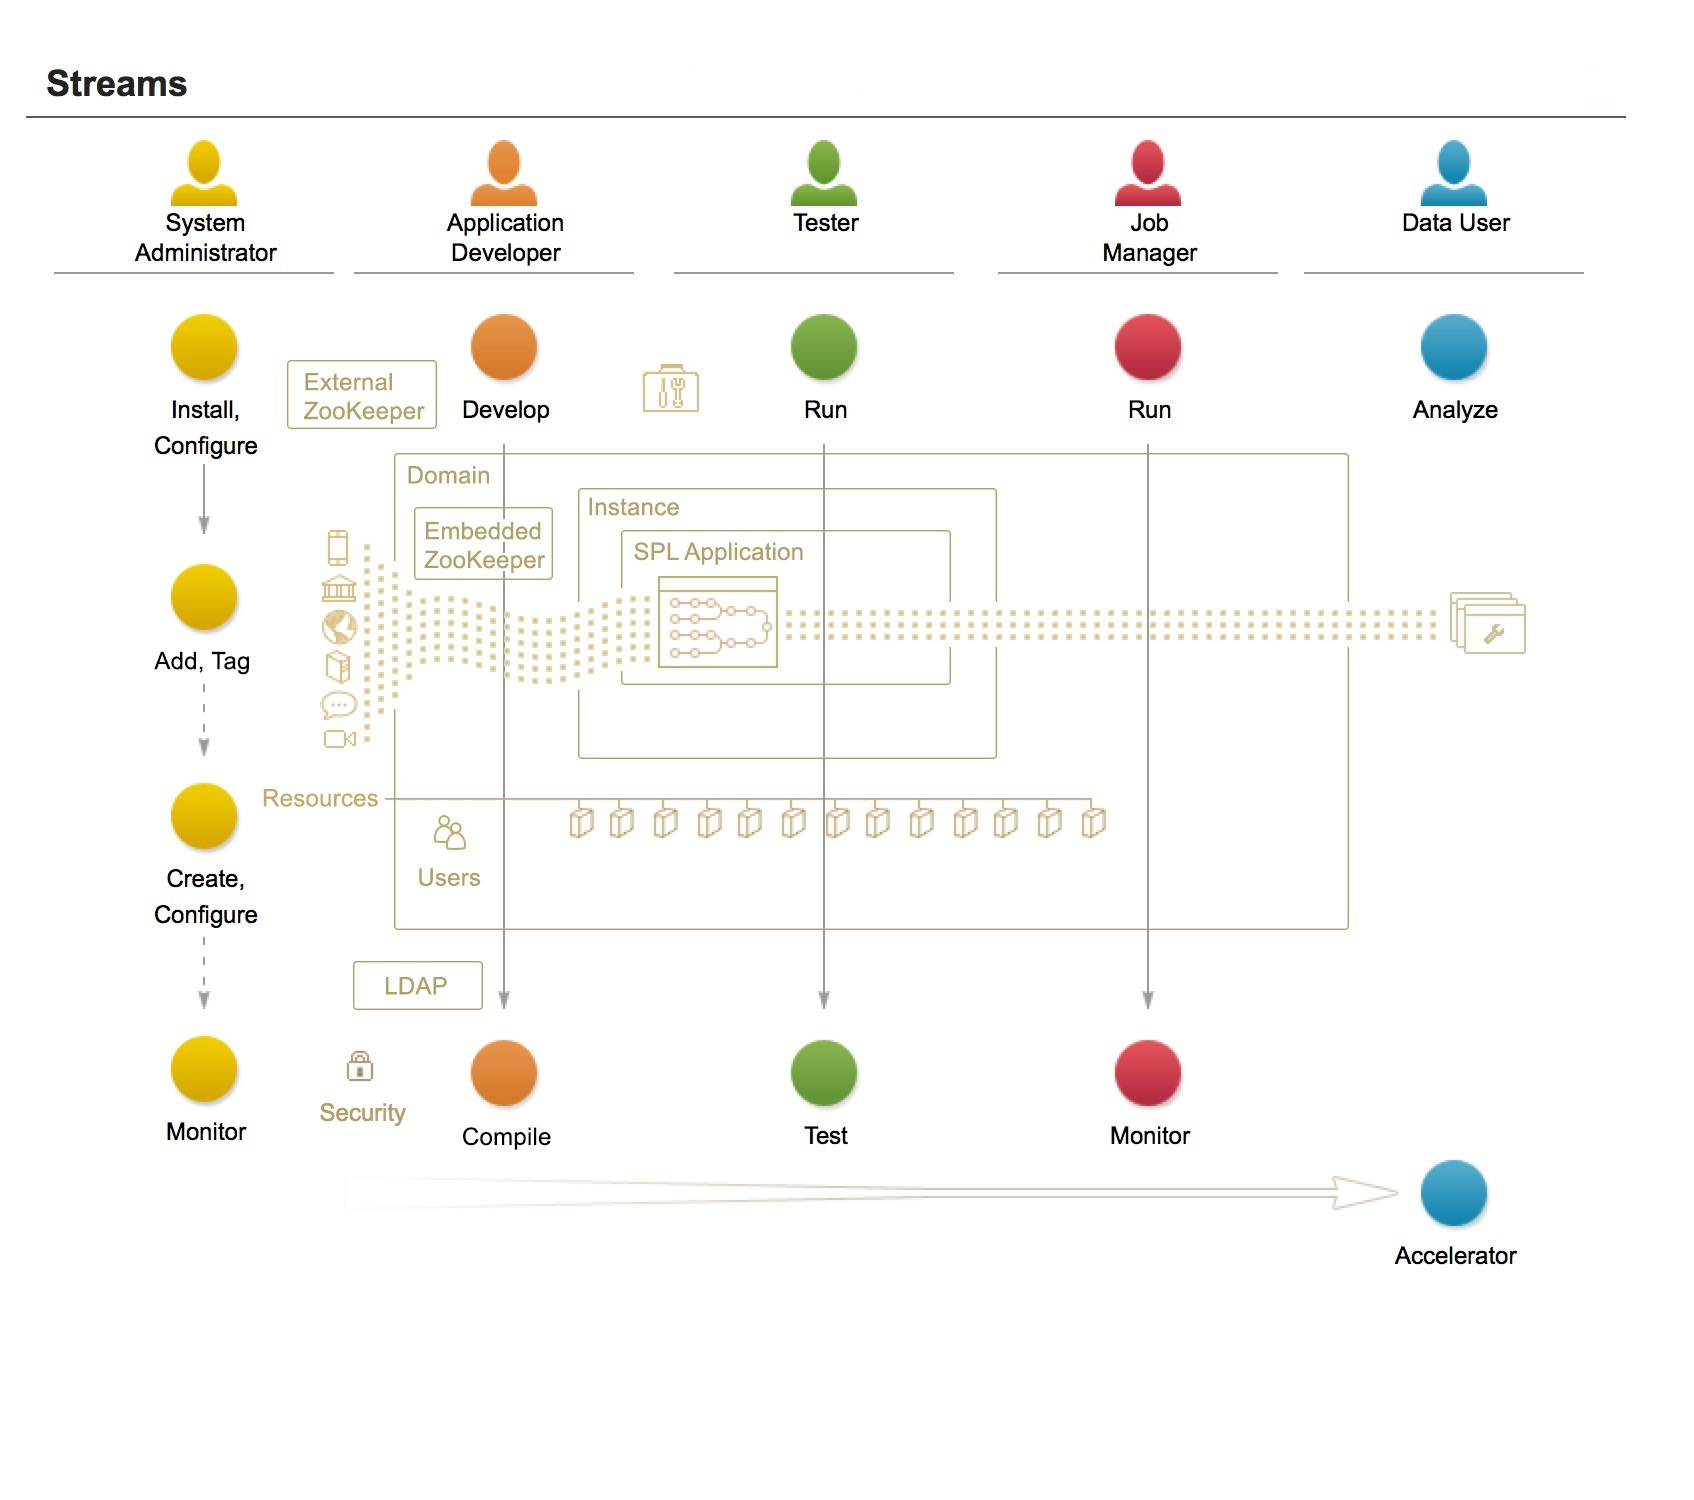
\includegraphics[width=1\linewidth]{figures/model.jpg}
	\caption{\cite{ibmdoc} IBM InfoSphere Streams}
	\label{fig:ibm}
\end{figure}


\subsection{Streaming for Line Simplification}
In this section we will discuss the current state of line simplification algorithm/problem in the context of stream processing.
The main problematic of this thesis is related to this problem because of that this subject will have a more in depth analysis.

\cite{abam2007streaming} as mentionned in this article, suppose we are tracking one, or maybe many,
moving objects. Each object is equipped with a device that
is continuously transmitting its position. Thus we are re-
ceiving a stream of data points that describes the path along
which the object moves. The goal is to maintain this path
for each object. We are interested in the scenario where we
are tracking the objects over a very long period of time, as
happens for instance when studying the migratory patterns
of animals. In this situation it may be undesirable or even
impossible to store the complete stream of data points. In-
stead we have to maintain an approximation of the input
path. This leads us to the following problem: we are receiving a (possibly infinite) stream $p0,p1,p2,...$ of points in
the plane, and we wish to maintain a simplification (of the
part of the path seen so far) that is as close to the original
path as possible, while using not more than a given (fixed)
amount of available storage.

\subsubsection{Formalization}
In this subsection we will formalize the problem of line simplification in a streaming mode based on the article \cite{abam2007streaming}.
To be able to state the problem we wish to solve and the results we obtain more precisely, we first introduce some terminology and definitions.
Let $p_0, p_1, \ldots$ be the given stream of input points. We use $P(n)$ to denote the path defined by the points
$p_0, p_1, \ldots, p_n$ - that is, the path connecting those points in order - and for any two points $p, q$ on the path we use
$P(p, q)$ to denote the subpath from $p$ to $q$. For two vertices $p_i, p_j$ we use $P(i, j)$ as a shorthand for $P\left(p_i, p_j\right)$.
A segment $p_i p_j$ with $i<j$ is called a link or sometimes a shortcut. Thus $P(n)$ consists of the links $p_{i-1} p_i$ for $0<i \leqslant n$.
We assume a function error is given that assigns a non-negative error to each link $p_i p_j$.
A $\ell$-simplification of $P(n)$ is a polygonal path $Q:=q_0, q_1, \ldots, q_k, q_{k+1}$ where
$k \leqslant \ell$ and $q_0=p_0$ and $q_{k+1}=p_n$, and $q_1, \ldots, q_k$ is a subsequence of
$p_1, \ldots, p_{n-1}$. The error of a simplification $Q$ for a given function error, denoted
$\operatorname{error}(Q)$, is defined as the maximum error of any of its links.

\subsubsection{Evaluation}
\cite{abam2007streaming}  Now consider an algorithm $\mathcal{A}:=\mathcal{A}(\ell)$ that maintains an $\ell$-simplification for the input stream $p_0, p_1, \ldots$,
for some given $\ell$. Let $Q_{\mathcal{A}}(n)$ denote the simplification that $\mathcal{A}$ produces for the path $P(n)$. Let $\operatorname{Opt}(\ell)$
denote an optimal off-line algorithm that produces an $\ell$-simplification. Thus $\operatorname{error}\left(Q_{O p t(\ell)}(n)\right)$ is the minimum possible
error of any $\ell-$ simplification of $P(n)$. We define the quality of $\mathcal{A}$ using the competitive ratio, as is standard for on-line algorithms.
We also allow resource augmentation. More precisely, we allow $\mathcal{A}$ to use a $2k$-simplification, but we compare the error of this simplification
to $Q_{O p t(k)}(n)$. (This is similar to Agarwal et al. \cite{agarwal2005near} who compare the quality of their solution to the min- $k$ problem for a given maximum error $\delta$
to the optimal value for maximum error $\delta / 2$.) Thus we define the competitive ratio of an algorithm $\mathcal{A}(2 k)$ as
$$
\text { competitive ratio of } \mathcal{A}(2 k):=\max _{n \geqslant 0} \frac{\operatorname{error}\left(Q_{\mathcal{A}(2 k)}(n)\right)}{\operatorname{error}\left(Q_{O p t(k)}(n)\right)},
$$
where $\frac{\operatorname{error}\left(Q_{\mathcal{A}(2 k)}(n)\right)}{\operatorname{error}\left(Q_{O p t(k)}(n)\right)}$ is defined as
1 if $\operatorname{error}\left(Q_{\mathcal{A}(2 k)}(n)\right)=$ $\operatorname{error}\left(Q_{O p t(k)}(n)\right)=0$.
We say that an algorithm is $c$ competitive if its competitive ratio is at most $c$.

\subsubsection{Algorithm}
We will discuss the existing algorithm for the line simplification in a streaming model. In the article \cite{abam2007streaming} they propose
the following algorithm. Our algorithm is quite simple. Suppose we have already handled the points $p_0, \ldots, p_n$.
(We assume $n>\ell+1$; until that moment we can simply use all points and have zero error.) Let $Q:=q_0, q_1, \ldots, q_{\ell}, q_{\ell+1}$
be the current simplification. Our algorithm will maintain a priority queue $\mathcal{Q}$ that stores the points $q_i$ with $1 \leqslant i \leqslant \ell$,
where the priority of a point is the error (as computed by the oracle) of the link $q_{i-1} q_{i+1}$. In other words, the priority of $q_i$ is
(an approximation of) the error that is incurred when $q_i$ is removed from the simplification. Now the next point $p_{n+1}$ is handled as follows:

\begin{enumerate}
	\item  Set $q_{\ell+2}:=p_{n+1}$, thus obtaining an $(\ell+1)$-simplification of $P(n+1)$.
	\item  Compute $\operatorname{error}^*\left(q_{\ell} q_{\ell+2}\right)$ and insert $q_{\ell+1}$ into $\mathcal{Q}$ with this error as priority.
	\item  Extract the point $q_s$ with minimum priority from $\mathcal{Q}$; remove $q_s$ from the simplification.
	\item  Update the priorities of $q_{s-1}$ and $q_{s+1}$ in $\mathcal{Q}$.
	
\end{enumerate}

As we can see the following algorithm is using the error function in order to correct the result in real-time. In the context of this thesis we will investigate a solution
that is based on the existing algorithm douglas-peucker to see if it is possible to maintain a simplified version of the trip using this algorithm.




\subsection{Moving Object Database}
In order to store the position of our tracking objects it is important to
search on moving object database as data output for this thesis.
\cite[Moving objects are objects that change their value or location
with time. These can be vehicles, persons, animals, aircarft, the air
temperature of a city, the fuel price in a certain gas station, etc.
The ubiquity of tracking devices and IoT technologies has resulted
in collecting massive amounts of data that describe the temporal
evolution of such objects and values. This creates opportunities
to build applications on this data, which in turn calls for building]{zimanyi2019mobilitydb}

As mentioned above the need for a specific database in order to have an efficient data storage.
In the context of this thesis we will focus on mobilityDB which is a Moving Object database that extends
PostgreSQL

\subsubsection{PostgreSQL}

\cite{postgresql} PostgreSQL is an object-relational database management system (ORDBMS) based on POSTGRES, Version 4.2,
developed at the University of California at Berkeley Computer Science Department. POSTGRES pioneered many
concepts that only became available in some commercial database systems much later.

PostgreSQL is an open-source descendant of this original Berkeley code. It supports a large part of the SQL standard
and offers many modern features:

\begin{itemize}
	
	\item complex queries
	\item foreign keys
	\item triggers
	\item updatable views
	\item transactional integrity
	\item multiversion concurrency control
\end{itemize}

Also, PostgreSQL can be extended by the user in many ways, for example by adding new

\begin{itemize}
	\item data types
	\item functions
	\item operators
	\item aggregate functions
	\item index methods
	\item procedural languages
\end{itemize}
And because of the liberal license, PostgreSQL can be used, modified, and distributed by anyone free of charge for any purpose, be it private, commercial, or academic.


\subsubsection{PostGIS}
\cite{marquez2015postgis} PostGIS represents a potent open-source instrument facilitating the creation of resilient spatial databases. Serving as the geographic extension of the PostgreSQL database management system, PostGIS enables the incorporation of geographic objects within data tables. These geographic objects are specialized data types designed for the storage of geographic positions or sets thereof, integrated seamlessly into lines or polygons. In essence, PostGIS emerges as a formidable tool, empowering users to manage intricate geographical data proficiently and to visually interrogate such data when employed in conjunction with graphical tools, exemplified by QGIS.

\subsubsection{MobilityDB}
MobilityDB uses the abstract data type approach of MOD implementations
\cite{guting2000foundation}. In an extensible relational database system this
amounts to adding user-defined types that can be used as attribute
types inside relations. MobilityDB defines in PostgreSQL and PostGIS
the temporal types: tgeompoint, tgeogpoint, tfloat, tint,
ttext, and tbool. These types encode functions from the time
domain to their corresponding base type domains. MobilityDB extends the existential
spatial database by adding a new dimension. It becomes more dynamics and respond to the need 
of processing moving object data. 


\chapter{Design}
\section{SQUISH-E}
In this section we introduce the SQUISH-E algorithm, present a pseudo-code and analyze its complexity. \\

The SQUISH-E algorithm compresses a trajectory \(T\) by utilizing two parameters, \(\lambda\) and \(\mu\), to strategically minimize the Synchronized Euclidean Distance (SED) error while achieving a specified compression ratio (\(\lambda\)). It operates by compressing \(T\) until further compression would result in an increase in SED error above \(\mu\), with a notable case being SQUISH-E(\(\lambda\)) where setting \(\mu\) to 0 focuses on minimizing SED error to achieve the compression ratio of \(\lambda\). In contrast, SQUISH-E(\(\mu\)) highlights a scenario where \(\lambda\) is set to 1, aiming to maximize the compression ratio without exceeding the SED error threshold defined by \(\mu\). A pivotal aspect of SQUISH-E is its use of a priority queue \(Q\), in which the priority of each point is determined by an upper bound on the SED error that could be introduced by its removal. This mechanism allows SQUISH-E to efficiently identify and remove the point with the lowest priority, i.e., the point whose removal would result in the least increase in SED error, in \(O(\log |Q|)\) time. This process effectively controls the growth of SED error, ensuring the algorithm's efficiency in compressing trajectory data while maintaining the integrity of the spatial information \cite{muckell2014compression}. In order to have a fully online algorithm SQUISH-E(\(\mu\)) is not taken into account and we only take into account SQUISH-E(\(\lambda\)). The error function is the same but in our implementation it could be a nice idea to compare different error function to find the best ones for some situation.

\subsection{Algorithm Pseudo-Code}
In this section we will present the pseudo-code of SQUISH-E algorithm used in our work. \\

\begin{algorithm}[H]
	\DontPrintSemicolon
	\KwIn{trajectory $T$, lower bound $\lambda$ on compression ratio}
	\KwOut{trajectory $T'$}
	$\beta \gets 4$ \tcp*{the initial capacity of $Q$ is 4}
	\ForEach{point $P_i \in T$}{
		\If{$\frac{i}{\lambda} \geq \beta$}{
			$\beta \gets \beta + 1$ \tcp*{increase the capacity of $Q$}
		}
		set\_priority($P_i, \infty, Q$) \tcp*{enqueue $P_i$ with the priority of $P_i$ being $\infty$}
		$\pi[P_i] \gets 0$\;
		\If{$i > 1$}{
			$succ[P_{i-1}] \gets P_i$ \tcp*{register $P_i$ as $P_{i-1}$'s closest successor}
			$pred[P_i] \gets P_{i-1}$ \tcp*{register $P_{i-1}$ as $P_i$'s closest predecessor}
			adjust\_priority($P_{i-1}, Q, pred, succ, \pi$) \tcp*{Algorithm 3}
		}
		\If{$|Q| = \beta$}{
			reduce($Q, pred, succ, \pi$) \tcp*{Algorithm 2}
		}
	}
	\Return{trajectory $T'$ comprising the points in $Q$ in the order reflected in the $succ$ map}
	\caption{SQUISH-E($T, \lambda$)}
	\label{alg:squish_e}
\end{algorithm}

In the algorithm \ref{alg:squish_e} we can analyze the time complexity. L'algorithme fonctionne de maniére itérationnelle en recevant un par un chaque point ce qui est pratique pour notre cas streaming. La complexité est donc au minima $O(n * max(O(set_priority),O(adjust_priority),O(reduce)) )$  

\newpage
\printbibliography
%\bibliography{reference}
%\bibliographystyle{abbrv}


\end{document}
